% Chapter 5: GARCH and Volatility
% Harvard-quality academic presentation
% Bachelor program, Bucharest University of Economic Studies

\documentclass[9pt, aspectratio=169, t]{beamer}

% Ensure content fits on slides
\setbeamersize{text margin left=8mm, text margin right=8mm}

%=============================================================================
% THEME AND STYLE CONFIGURATION
%=============================================================================
\usetheme{default}
% Using default theme for clean header/footer control

% Color Palette (matching Redispatch PDF)
\definecolor{MainBlue}{RGB}{26, 58, 110}
\definecolor{AccentBlue}{RGB}{26, 58, 110}
\definecolor{IDAred}{RGB}{205, 0, 0}
\definecolor{DarkGray}{RGB}{51, 51, 51}
\definecolor{MediumGray}{RGB}{128, 128, 128}
\definecolor{LightGray}{RGB}{248, 248, 248}
\definecolor{VeryLightGray}{RGB}{235, 235, 235}
\definecolor{KeynoteGray}{RGB}{218, 218, 218}
\definecolor{SectionGray}{RGB}{120, 120, 120}
\definecolor{FooterGray}{RGB}{100, 100, 100}
\definecolor{Crimson}{RGB}{220, 53, 69}
\definecolor{Forest}{RGB}{46, 125, 50}
\definecolor{Amber}{RGB}{181, 133, 63}
\definecolor{Orange}{RGB}{230, 126, 34}
\definecolor{Purple}{RGB}{142, 68, 173}

% Gradient background (exact Keynote 315° gradient: white to RGB 218,218,218)
\setbeamertemplate{background}{%
    \begin{tikzpicture}[remember picture, overlay]
        \shade[shading=axis, shading angle=315,
        top color=white, bottom color=KeynoteGray]
        (current page.south west) rectangle (current page.north east);
    \end{tikzpicture}%
}
% Fallback solid color for compatibility
\setbeamercolor{background canvas}{bg=}

\setbeamercolor{palette primary}{bg=MainBlue, fg=white}
\setbeamercolor{palette secondary}{bg=MainBlue!85, fg=white}
\setbeamercolor{palette tertiary}{bg=MainBlue!70, fg=white}
\setbeamercolor{structure}{fg=MainBlue}
\setbeamercolor{title}{fg=IDAred}
\setbeamercolor{frametitle}{fg=IDAred, bg=}
\setbeamercolor{block title}{bg=MainBlue, fg=white}
\setbeamercolor{block body}{bg=VeryLightGray, fg=DarkGray}
\setbeamercolor{block title alerted}{bg=Crimson, fg=white}
\setbeamercolor{block body alerted}{bg=Crimson!8, fg=DarkGray}
\setbeamercolor{block title example}{bg=Forest, fg=white}
\setbeamercolor{block body example}{bg=Forest!8, fg=DarkGray}
\setbeamercolor{item}{fg=MainBlue}

% Footer colors (override Madrid theme blue)
\setbeamercolor{author in head/foot}{fg=FooterGray, bg=}
\setbeamercolor{title in head/foot}{fg=FooterGray, bg=}
\setbeamercolor{date in head/foot}{fg=FooterGray, bg=}
\setbeamercolor{section in head/foot}{fg=FooterGray, bg=}
\setbeamercolor{subsection in head/foot}{fg=FooterGray, bg=}

% Bullet styles (apply everywhere including blocks)
\setbeamertemplate{itemize item}{\color{MainBlue}$\boxdot$}
\setbeamertemplate{itemize subitem}{\color{MainBlue}$\blacktriangleright$}
\setbeamertemplate{itemize subsubitem}{\color{MainBlue}\tiny$\bullet$}
\setbeamertemplate{itemize/enumerate body begin}{\normalsize}
\setbeamertemplate{itemize/enumerate subbody begin}{\normalsize}

% Item spacing
\setlength{\leftmargini}{1.5em}
\setlength{\leftmarginii}{1.5em}

\setbeamertemplate{navigation symbols}{}

% TOC with bullets
\setbeamertemplate{section in toc}{\color{MainBlue}$\boxdot$\hspace{0.5em}\inserttocsection}

%=============================================================================
% CUSTOM HEADLINE
%=============================================================================
\setbeamertemplate{headline}{%
    \vskip10pt%
    \hbox to \paperwidth{%
        \hskip0.5cm%
        {\small\color{FooterGray}\renewcommand{\hyperlink}[2]{##2}\insertsectionhead}%
        \hfill%
        \textcolor{FooterGray}{\small\insertframenumber}%
        \hskip0.5cm%
    }%
    \vskip4pt%
    {\color{FooterGray}\hrule height 0.4pt}%
}

%=============================================================================
% CUSTOM FOOTER
%=============================================================================
\usepackage{fontawesome5}

\setbeamertemplate{footline}{%
    {\color{FooterGray}\hrule height 0.4pt}%
    \vskip4pt%
    \hbox to \paperwidth{%
        \hskip0.5cm%
        \textcolor{FooterGray}{\small Time Series Analysis and Forecasting}%
        \hfill%
        \raisebox{-0.1em}{%
            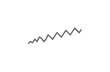
\begin{tikzpicture}[x=0.08em, y=0.08em, line width=0.4pt]
                \draw[FooterGray] (0,3) -- (1,4) -- (2,3.5) -- (3,5) -- (4,4) -- (5,6) -- (6,5.5) -- (7,4) -- (8,5) -- (9,7) -- (10,6) -- (11,5) -- (12,6.5) -- (13,8) -- (14,7) -- (15,6) -- (16,7.5) -- (17,9) -- (18,8) -- (19,7) -- (20,8.5) -- (21,10) -- (22,9) -- (23,8) -- (24,9.5);
            \end{tikzpicture}%
        }%
        \hskip0.5cm%
    }%
    \vskip6pt%
}

%=============================================================================
% PACKAGES
%=============================================================================
\usepackage[utf8]{inputenc}
\usepackage[T1]{fontenc}
\usepackage{amsmath, amssymb, amsthm}
\usepackage{mathtools}
\usepackage{bm}
\usepackage{tikz}
\usetikzlibrary{arrows.meta, positioning, shapes, calc, decorations.pathreplacing, shadings}
\usepackage{booktabs}
\usepackage{multirow}
\usepackage{array}
\usepackage{graphicx}
\usepackage{hyperref}
\usepackage{colortbl}
\hypersetup{colorlinks=true, linkcolor=MainBlue, urlcolor=MainBlue}
\graphicspath{{../logos/}{../charts/}}

%=============================================================================
% QUANTLET COMMAND
%=============================================================================
\newcommand{\quantlet}[2]{%
    \begin{tikzpicture}[remember picture, overlay]
        \node[anchor=south east, inner sep=0pt] at ([xshift=-0.5cm, yshift=0.75cm]current page.south east) {%
            \href{#2}{%
                \raisebox{-0.1em}{\includegraphics[height=0.8em]{ql_logo.png}}%
                \textcolor{MainBlue}{\scriptsize\ #1}%
            }%
        };
    \end{tikzpicture}%
}

%=============================================================================
% CUSTOM TITLE PAGE
%=============================================================================
\defbeamertemplate*{title page}{hybrid}[1][]
{
    \vspace{0.2cm}
    % Logos row - top header (with clickable links)
    \begin{center}
        \href{https://www.ase.ro}{\includegraphics[height=1.0cm]{ase_logo.png}}\hspace{0.3cm}%
        \href{https://theida.net}{\includegraphics[height=1.0cm]{ida_logo.png}}\hspace{0.3cm}%
        \href{https://blockchain-research-center.com}{\includegraphics[height=1.0cm]{brc_logo.png}}\hspace{0.3cm}%
        \href{https://www.ai4efin.ase.ro}{\includegraphics[height=1.0cm]{ai4efin_logo.png}}\hspace{0.3cm}%
        \href{https://ipe.ro/new}{\includegraphics[height=1.0cm]{acad_logo.png}}\hspace{0.3cm}%
        \href{https://www.digital-finance-msca.com}{\includegraphics[height=1.0cm]{msca_logo.png}}%
    \end{center}

    \vspace{0.6cm}

    % Main title with Q logos on sides (with clickable links)
    \begin{center}
        \begin{minipage}{0.1\textwidth}
            \centering
            \href{https://quantlet.com}{\includegraphics[height=1.1cm]{ql_logo.png}}
        \end{minipage}%
        \begin{minipage}{0.78\textwidth}
            \centering
            {\LARGE\bfseries\usebeamercolor[fg]{title}\inserttitle}

            \vspace{0.3cm}

            {\usebeamerfont{subtitle}\usebeamercolor[fg]{title}\insertsubtitle}
        \end{minipage}%
        \begin{minipage}{0.1\textwidth}
            \centering
            \href{https://quantinar.com}{\includegraphics[height=1.1cm]{qr_logo.png}}
        \end{minipage}
    \end{center}

    \vspace{0.6cm}

    % Authors (left aligned)
    \hspace{0.5cm}{\usebeamerfont{author}\insertauthor}

    \vspace{0.3cm}

    % Institute/Affiliations (left aligned)
    \hspace{0.5cm}\begin{minipage}[t]{0.9\textwidth}
        \raggedright\small\insertinstitute
    \end{minipage}
}

%=============================================================================
% THEOREM ENVIRONMENTS
%=============================================================================
\theoremstyle{definition}
\setbeamertemplate{theorems}[numbered]
\newtheorem{defn}{Definition}
\newtheorem{thm}{Theorem}
\newtheorem{prop}{Proposition}
\newtheorem{rmk}{Remark}

%=============================================================================
% CUSTOM COMMANDS
%=============================================================================
\newcommand{\E}{\mathbb{E}}
\newcommand{\Var}{\text{Var}}
\newcommand{\Cov}{\text{Cov}}
\newcommand{\Corr}{\text{Corr}}
\newcommand{\R}{\mathbb{R}}
\newcommand{\N}{\mathbb{N}}
\newcommand{\Z}{\mathbb{Z}}
\newcommand{\B}{\mathbf{B}}
\newcommand{\imark}{\textcolor{MainBlue}{\textbullet}}
\newcommand{\RMSE}{\text{RMSE}}
\newcommand{\MAE}{\text{MAE}}
\newcommand{\MAPE}{\text{MAPE}}

%=============================================================================
% TITLE INFORMATION
%=============================================================================
\title[Time Series Analysis]{Time Series Analysis and Forecasting}
\subtitle{Chapter 5: GARCH and Volatility}
\author[D.T. Pele]{Daniel Traian PELE}
\institute{Bucharest University of Economic Studies\\
IDA Institute Digital Assets\\
Blockchain Research Center\\
AI4EFin Artificial Intelligence for Energy Finance\\
Romanian Academy, Institute for Economic Forecasting\\
MSCA Digital Finance}
\date{}

\begin{document}

% Title page (no header/footer)
{
\setbeamertemplate{headline}{}
\setbeamertemplate{footline}{}
\begin{frame}
    \titlepage
\end{frame}
}

%=============================================================================
% TABLE OF CONTENTS
%=============================================================================
\begin{frame}{Outline}
    \tableofcontents
\end{frame}

%=============================================================================
% SECTION 1: INTRODUCTION TO VOLATILITY
%=============================================================================
\section{Introduction to Volatility Modeling}

\begin{frame}{Why Model Volatility?}
    \begin{block}{Empirical Observations in Financial Series}
        \begin{itemize}
            \item Financial returns exhibit \textbf{volatility clustering} --- periods of high volatility tend to be followed by periods of high volatility
            \item The distribution of returns has \textbf{fat tails} (leptokurtosis)
            \item Return correlation is nearly zero, but correlation of squares is significant
            \item Volatility responds \textbf{asymmetrically} to shocks (leverage effect)
        \end{itemize}
    \end{block}

    \vspace{0.3cm}

    \begin{alertblock}{Limitation of ARIMA Models}
        ARIMA models assume \textbf{constant variance} (homoskedasticity), which is not realistic for financial series!
    \end{alertblock}
\end{frame}

\begin{frame}{Volatility Clustering}
    \begin{center}
        \includegraphics[width=0.78\textwidth, height=0.55\textheight, keepaspectratio]{garch_volatility_clustering.pdf}
    \end{center}
    \vspace{-0.2cm}
    \begin{itemize}
        \item High volatility periods are followed by high volatility; calm by calm
        \item This suggests that \textbf{conditional variance} is predictable
    \end{itemize}
    \quantlet{TSA\_garch\_volatility\_clustering}{https://github.com/QuantLet/TSA/tree/main/TSA_garch_volatility_clustering}
\end{frame}

\begin{frame}{Stylized Facts of Financial Returns}
    \begin{columns}[T]
        \begin{column}{0.48\textwidth}
            \begin{block}{Observed Properties}
                \begin{enumerate}
                    \item \textbf{No autocorrelation} in returns
                    \item \textbf{Autocorrelation} in $r_t^2$, $|r_t|$
                    \item \textbf{Fat tails} (kurtosis $> 3$)
                    \item \textbf{Leverage effect}
                    \item \textbf{Volatility clustering}
                \end{enumerate}
            \end{block}
        \end{column}
        \begin{column}{0.52\textwidth}
            \begin{center}
                \includegraphics[width=\textwidth, height=0.65\textheight, keepaspectratio]{garch_stylized_facts.pdf}
            \end{center}
        \end{column}
    \end{columns}
    \quantlet{TSA\_garch\_stylized\_facts}{https://github.com/QuantLet/TSA/tree/main/TSA_garch_stylized_facts}
\end{frame}

\begin{frame}{Conditional Heteroskedasticity}
    \begin{defn}[Conditional Variance]
        For return series $\{r_t\}$, the \textbf{conditional variance} at time $t$ is:
        $\sigma_t^2 = \Var(r_t | \mathcal{F}_{t-1}) = \E[(r_t - \mu_t)^2 | \mathcal{F}_{t-1}]$
        where $\mathcal{F}_{t-1}$ is the information available up to time $t-1$.
    \end{defn}

    \vspace{0.2cm}

    \begin{block}{General Model}
        $r_t = \mu_t + \varepsilon_t$, \quad $\varepsilon_t = \sigma_t z_t$, \quad $z_t \sim \text{i.i.d.}(0, 1)$
        \begin{itemize}
            \item $\mu_t$ = conditional mean (ARMA); \quad $\sigma_t^2$ = conditional variance (GARCH)
            \item $z_t$ = standardized innovations (Normal, Student-t, GED)
        \end{itemize}
    \end{block}
\end{frame}

%=============================================================================
% SECTION 2: ARCH MODEL
%=============================================================================
\section{The ARCH Model}

\begin{frame}{The ARCH(q) Model --- Engle (1982)}
    \begin{defn}[ARCH(q)]
        The \textbf{Autoregressive Conditional Heteroskedasticity} model of order $q$:
        \[
            \varepsilon_t = \sigma_t z_t, \quad z_t \sim \text{i.i.d.}(0, 1), \quad
            \sigma_t^2 = \omega + \sum_{i=1}^{q} \alpha_i \varepsilon_{t-i}^2
        \]
    \end{defn}

    \vspace{0.2cm}

    \begin{block}{Stationarity Restrictions}
        \begin{itemize}
            \item $\omega > 0$ (positive base variance), \quad $\alpha_i \geq 0$ (non-negativity)
            \item $\sum_{i=1}^{q} \alpha_i < 1$ (stationarity)
        \end{itemize}
    \end{block}

    \begin{rmk}
        Robert Engle received the \textbf{Nobel Prize in Economics} in 2003 for developing the ARCH model!
    \end{rmk}
\end{frame}

\begin{frame}{Properties of the ARCH(1) Model}
    \begin{block}{ARCH(1): $\sigma_t^2 = \omega + \alpha_1 \varepsilon_{t-1}^2$}
        \begin{itemize}
            \item \textbf{Unconditional variance}: $\E[\varepsilon_t^2] = \dfrac{\omega}{1 - \alpha_1}$ (if $\alpha_1 < 1$)
            \item \textbf{Kurtosis}: $\kappa = 3 \cdot \dfrac{1 - \alpha_1^2}{1 - 3\alpha_1^2}$ (if $\alpha_1^2 < 1/3$)
            \item Kurtosis $> 3$ for $\alpha_1 > 0$ $\Rightarrow$ \textbf{fat tails}!
        \end{itemize}
    \end{block}

    \vspace{0.3cm}

    \begin{exampleblock}{Numerical Example}
        If $\omega = 0.0001$ and $\alpha_1 = 0.3$:
        \begin{itemize}
            \item Unconditional variance: $\sigma^2 = \frac{0.0001}{1 - 0.3} = 0.000143$
            \item Kurtosis: $\kappa = 3 \cdot \frac{1 - 0.09}{1 - 0.27} = 3.74 > 3$
        \end{itemize}
    \end{exampleblock}
\end{frame}

\begin{frame}{Testing for ARCH Effects}
    \begin{block}{Engle's Test for ARCH Effects}
        \textbf{Procedure}:
        \begin{enumerate}
            \item Estimate the mean model and obtain residuals $\hat{\varepsilon}_t$
            \item Calculate $\hat{\varepsilon}_t^2$
            \item Regress $\hat{\varepsilon}_t^2$ on its lags:
            \[
                \hat{\varepsilon}_t^2 = \beta_0 + \beta_1 \hat{\varepsilon}_{t-1}^2 + \cdots + \beta_q \hat{\varepsilon}_{t-q}^2 + u_t
            \]
            \item Calculate the statistic $LM = T \cdot R^2 \sim \chi^2(q)$
        \end{enumerate}
    \end{block}

    \vspace{0.3cm}

    \begin{alertblock}{Hypotheses}
        \begin{itemize}
            \item $H_0$: No ARCH effects ($\alpha_1 = \cdots = \alpha_q = 0$)
            \item $H_1$: ARCH effects present (at least one $\alpha_i \neq 0$)
        \end{itemize}
    \end{alertblock}
\end{frame}

\begin{frame}{Limitations of the ARCH Model}
    \begin{alertblock}{Practical Problems}
        \begin{enumerate}
            \item \textbf{High order} --- many lags are usually needed (large $q$)
            \item \textbf{Many parameters} --- estimation difficulties
            \item \textbf{Non-negativity constraints} --- difficult to impose for large $q$
            \item \textbf{Does not capture persistence} --- observed volatility is very persistent
        \end{enumerate}
    \end{alertblock}

    \vspace{0.5cm}

    \begin{block}{The Solution}
        \textbf{The GARCH Model} --- introduces lags of conditional variance to capture persistence with fewer parameters!
    \end{block}
\end{frame}

%=============================================================================
% SECTION 3: GARCH MODEL
%=============================================================================
\section{The GARCH Model}

\begin{frame}{The GARCH(p,q) Model --- Bollerslev (1986)}
    \begin{defn}[GARCH(p,q)]
        The \textbf{Generalized ARCH} model:
        \[
            \varepsilon_t = \sigma_t z_t, \quad z_t \sim \text{i.i.d.}(0, 1)
        \]
        \[
            \sigma_t^2 = \omega + \sum_{i=1}^{q} \alpha_i \varepsilon_{t-i}^2 + \sum_{j=1}^{p} \beta_j \sigma_{t-j}^2
        \]
    \end{defn}

    \vspace{0.3cm}

    \begin{block}{Interpretation}
        \begin{itemize}
            \item $\omega$ = base level of volatility
            \item $\alpha_i$ = reaction to recent shocks (news coefficients)
            \item $\beta_j$ = volatility persistence (memory)
            \item $\alpha + \beta$ = total persistence
        \end{itemize}
    \end{block}
\end{frame}

\begin{frame}{The GARCH(1,1) Model}
    \begin{block}{The Most Popular Volatility Model}
        $\sigma_t^2 = \omega + \alpha \varepsilon_{t-1}^2 + \beta \sigma_{t-1}^2$
    \end{block}

    \begin{columns}[T]
        \begin{column}{0.48\textwidth}
            \begin{block}{Restrictions \& Properties}
                \begin{itemize}
                    \item $\omega > 0$, $\alpha \geq 0$, $\beta \geq 0$
                    \item $\alpha + \beta < 1$ (stationarity)
                    \item $\bar{\sigma}^2 = \frac{\omega}{1 - \alpha - \beta}$
                    \item Half-life: $HL = \frac{\ln(0.5)}{\ln(\alpha + \beta)}$
                \end{itemize}
            \end{block}
        \end{column}
        \begin{column}{0.52\textwidth}
            \begin{center}
                \includegraphics[width=\textwidth, height=0.55\textheight, keepaspectratio]{garch_conditional_variance.pdf}
            \end{center}
        \end{column}
    \end{columns}
    \quantlet{TSA\_garch\_conditional\_variance}{https://github.com/QuantLet/TSA/tree/main/TSA_garch_conditional_variance}
\end{frame}

\begin{frame}{GARCH(1,1) as ARMA for $\varepsilon_t^2$}
    \begin{block}{ARMA(1,1) Representation}
        Define $\nu_t = \varepsilon_t^2 - \sigma_t^2$ (variance shock). Then:
        \[
            \varepsilon_t^2 = \omega + (\alpha + \beta) \varepsilon_{t-1}^2 + \nu_t - \beta \nu_{t-1}
        \]

        This is an \textbf{ARMA(1,1)} for $\varepsilon_t^2$!
    \end{block}

    \vspace{0.3cm}

    \begin{exampleblock}{Implications}
        \begin{itemize}
            \item ACF of $\varepsilon_t^2$ decays exponentially (like ARMA)
            \item Persistence is given by $\alpha + \beta$
            \item PACF can help identify the order
        \end{itemize}
    \end{exampleblock}
\end{frame}

\begin{frame}{Estimation of GARCH Models}
    \begin{block}{Maximum Likelihood Estimation (MLE)}
        Log-likelihood (normal): $\ell(\theta) = -\frac{T}{2} \ln(2\pi) - \frac{1}{2} \sum_{t=1}^{T} \left[ \ln(\sigma_t^2) + \frac{\varepsilon_t^2}{\sigma_t^2} \right]$
    \end{block}

    \vspace{0.2cm}

    \begin{block}{Alternative Distributions for $z_t$}
        \begin{itemize}
            \item \textbf{Student-t}: captures fat tails --- most common choice
            \item \textbf{GED}: flexibility for kurtosis
            \item \textbf{Skewed Student-t}: asymmetry and fat tails
        \end{itemize}
    \end{block}

    \vspace{0.2cm}

    \begin{alertblock}{Practical Note}
        Student-t distribution typically provides better fit for financial returns due to fat tails (kurtosis $> 3$).
    \end{alertblock}
\end{frame}

\begin{frame}{Typical Values for GARCH(1,1)}
    \begin{center}
        \begin{tabular}{lccc}
            \toprule
            \textbf{Series} & $\bm{\alpha}$ & $\bm{\beta}$ & $\bm{\alpha + \beta}$ \\
            \midrule
            S\&P 500 daily & 0.05--0.10 & 0.85--0.95 & 0.95--0.99 \\
            EUR/USD daily & 0.03--0.08 & 0.90--0.95 & 0.95--0.99 \\
            Bitcoin daily & 0.10--0.20 & 0.75--0.85 & 0.90--0.98 \\
            Bonds & 0.02--0.05 & 0.90--0.97 & 0.95--0.99 \\
            \bottomrule
        \end{tabular}
    \end{center}

    \vspace{0.5cm}

    \begin{alertblock}{Observations}
        \begin{itemize}
            \item $\alpha + \beta$ close to 1 $\Rightarrow$ \textbf{very persistent volatility}
            \item Small $\alpha$, large $\beta$ $\Rightarrow$ slow reaction to shocks, long memory
            \item Bitcoin: larger $\alpha$ $\Rightarrow$ faster reaction to news
        \end{itemize}
    \end{alertblock}
\end{frame}

\begin{frame}{IGARCH --- Integrated GARCH}
    \begin{defn}[IGARCH(1,1)]
        When $\alpha + \beta = 1$:
        \[
            \sigma_t^2 = \omega + \alpha \varepsilon_{t-1}^2 + (1 - \alpha) \sigma_{t-1}^2
        \]
    \end{defn}

    \vspace{0.3cm}

    \begin{block}{Properties}
        \begin{itemize}
            \item Unconditional variance does not exist (infinite)
            \item Shocks have \textbf{permanent} effect on volatility
            \item Used for series with extreme persistence
            \item Useful for \textbf{RiskMetrics} (J.P. Morgan): $\alpha = 0.06$, $\beta = 0.94$
        \end{itemize}
    \end{block}

    \begin{rmk}
        IGARCH is analogous to a unit root in variance!
    \end{rmk}
\end{frame}

%=============================================================================
% SECTION 4: ASYMMETRIC GARCH MODELS
%=============================================================================
\section{Asymmetric GARCH Models}

\begin{frame}{Leverage Effect}
    \begin{center}
        \includegraphics[width=0.65\textwidth, height=0.48\textheight, keepaspectratio]{garch_leverage_effect.pdf}
    \end{center}
    \vspace{-0.2cm}
    \begin{block}{Definition}
        \textbf{Leverage effect}: Negative shocks increase volatility \textbf{more} than positive shocks.
    \end{block}

    \begin{alertblock}{Problem with Standard GARCH}
        GARCH depends on $\varepsilon_{t-1}^2$, treating positive and negative shocks \textbf{symmetrically}!
    \end{alertblock}
    \quantlet{TSA\_garch\_leverage\_effect}{https://github.com/QuantLet/TSA/tree/main/TSA_garch_leverage_effect}
\end{frame}

\begin{frame}{The EGARCH Model --- Nelson (1991)}
    \begin{defn}[EGARCH(1,1)]
        \textbf{Exponential GARCH}:
        \[
            \ln(\sigma_t^2) = \omega + \alpha \left( |z_{t-1}| - \E[|z_{t-1}|] \right) + \gamma z_{t-1} + \beta \ln(\sigma_{t-1}^2)
        \]
        where $z_t = \varepsilon_t / \sigma_t$.
    \end{defn}

    \vspace{0.3cm}

    \begin{block}{EGARCH Advantages}
        \begin{itemize}
            \item \textbf{No non-negativity constraints required} --- models $\ln(\sigma_t^2)$
            \item \textbf{Captures leverage effect} through parameter $\gamma$
            \begin{itemize}
                \item $\gamma < 0$: negative shocks $\Rightarrow$ higher volatility
                \item $\gamma = 0$: symmetric effect (like GARCH)
            \end{itemize}
            \item Persistence is given by $\beta$
        \end{itemize}
    \end{block}
\end{frame}

\begin{frame}{News Impact Curve --- EGARCH}
    \begin{center}
        \includegraphics[width=0.68\textwidth, height=0.52\textheight, keepaspectratio]{garch_news_impact_curve.pdf}
    \end{center}
    \vspace{-0.2cm}
    \begin{block}{Interpretation}
        \textbf{News Impact Curve}: shows how $\sigma_{t+1}^2$ depends on shock $\varepsilon_t$, holding $\sigma_t^2$ constant.
    \end{block}
    \quantlet{TSA\_garch\_news\_impact\_curve}{https://github.com/QuantLet/TSA/tree/main/TSA_garch_news_impact_curve}
\end{frame}

\begin{frame}{The GJR-GARCH Model}
    \begin{defn}[GJR-GARCH(1,1)]
        Glosten, Jagannathan \& Runkle (1993):
        $\sigma_t^2 = \omega + \alpha \varepsilon_{t-1}^2 + \gamma \varepsilon_{t-1}^2 \cdot I_{t-1} + \beta \sigma_{t-1}^2$
        where $I_{t-1} = 1$ if $\varepsilon_{t-1} < 0$, else $0$.
    \end{defn}

    \vspace{0.2cm}

    \begin{block}{Interpretation}
        \begin{itemize}
            \item Positive shocks: impact = $\alpha$; \quad Negative shocks: impact = $\alpha + \gamma$
            \item Leverage effect present if $\gamma > 0$
            \item Stationarity: $\alpha + \gamma/2 + \beta < 1$
        \end{itemize}
    \end{block}
\end{frame}

\begin{frame}{TGARCH --- Threshold GARCH}
    \begin{defn}[TGARCH(1,1)]
        Zakoian (1994) models standard deviation:
        $\sigma_t = \omega + \alpha^+ \varepsilon_{t-1}^+ + \alpha^- \varepsilon_{t-1}^- + \beta \sigma_{t-1}$
    \end{defn}

    \vspace{0.2cm}

    \begin{block}{Comparison of Asymmetric Models}
        \begin{center}
            \small
            \begin{tabular}{lcc}
                \toprule
                \textbf{Model} & \textbf{Specification} & \textbf{Leverage} \\
                \midrule
                GARCH & $\sigma_t^2$ & No \\
                EGARCH & $\ln(\sigma_t^2)$ & Yes ($\gamma < 0$) \\
                GJR-GARCH & $\sigma_t^2$ with indicator & Yes ($\gamma > 0$) \\
                TGARCH & $\sigma_t$ & Yes ($\alpha^- > \alpha^+$) \\
                \bottomrule
            \end{tabular}
        \end{center}
    \end{block}
\end{frame}

%=============================================================================
% SECTION 5: MODEL SELECTION AND DIAGNOSTICS
%=============================================================================
\section{Model Selection and Diagnostics}

\begin{frame}{Order Selection}
    \begin{block}{Information Criteria}
        \begin{itemize}
            \item \textbf{AIC} = $-2\ell + 2k$
            \item \textbf{BIC} = $-2\ell + k \ln(T)$
            \item \textbf{HQIC} = $-2\ell + 2k \ln(\ln(T))$
        \end{itemize}
        where $\ell$ = maximized log-likelihood, $k$ = number of parameters.
    \end{block}

    \vspace{0.3cm}

    \begin{alertblock}{Practical Recommendations}
        \begin{itemize}
            \item GARCH(1,1) is sufficient in \textbf{90\% of cases}
            \item Check if asymmetric model significantly improves fit
            \item Choose innovation distribution that minimizes AIC/BIC
        \end{itemize}
    \end{alertblock}
\end{frame}

\begin{frame}{GARCH Model Diagnostics}
    \begin{block}{Standardized Residuals}
        \[
            \hat{z}_t = \frac{\hat{\varepsilon}_t}{\hat{\sigma}_t}
        \]

        If the model is correctly specified, $\hat{z}_t$ should be i.i.d.(0,1).
    \end{block}

    \vspace{0.3cm}

    \begin{block}{Diagnostic Checks}
        \begin{enumerate}
            \item \textbf{Ljung-Box on $\hat{z}_t$}: check absence of autocorrelation in mean
            \item \textbf{Ljung-Box on $\hat{z}_t^2$}: check absence of residual ARCH effects
            \item \textbf{ARCH-LM test on $\hat{z}_t$}: confirm absence of heteroskedasticity
            \item \textbf{Histogram + QQ-plot}: verify assumed distribution
        \end{enumerate}
    \end{block}
\end{frame}

\begin{frame}{Diagnostic Example}
    \begin{center}
        \includegraphics[width=0.72\textwidth, height=0.68\textheight, keepaspectratio]{garch_diagnostics.pdf}
    \end{center}
    \quantlet{TSA\_garch\_diagnostics}{https://github.com/QuantLet/TSA/tree/main/TSA_garch_diagnostics}
\end{frame}

%=============================================================================
% SECTION 6: FORECASTING VOLATILITY
%=============================================================================
\section{Volatility Forecasting}

\begin{frame}{Forecasting with GARCH(1,1)}
    \begin{block}{One-Step-Ahead Forecast}
        $\hat{\sigma}_{T+1}^2 = \omega + \alpha \varepsilon_T^2 + \beta \sigma_T^2$
    \end{block}

    \begin{block}{Multi-Step Forecast}
        For $h > 1$: $\E_T[\sigma_{T+h}^2] = \bar{\sigma}^2 + (\alpha + \beta)^{h-1} (\sigma_{T+1}^2 - \bar{\sigma}^2)$
        where $\bar{\sigma}^2 = \frac{\omega}{1 - \alpha - \beta}$ = unconditional variance.
    \end{block}

    \vspace{0.2cm}

    \begin{exampleblock}{Convergence}
        $\lim_{h \to \infty} \E_T[\sigma_{T+h}^2] = \bar{\sigma}^2$ --- forecast converges to unconditional variance!
    \end{exampleblock}
\end{frame}

\begin{frame}{Volatility Forecast --- Visualization}
    \begin{center}
        \includegraphics[width=0.75\textwidth, height=0.55\textheight, keepaspectratio]{garch_forecast.pdf}
    \end{center}
    \vspace{-0.2cm}
    \begin{itemize}
        \item Forecast converges exponentially to $\bar{\sigma}^2$; speed depends on $\alpha + \beta$
        \item The closer $\alpha + \beta$ is to 1, the slower the convergence
    \end{itemize}
    \quantlet{TSA\_garch\_forecast}{https://github.com/QuantLet/TSA/tree/main/TSA_garch_forecast}
\end{frame}

\begin{frame}{Applications of Volatility Forecasting}
    \begin{columns}[T]
        \begin{column}{0.5\textwidth}
            \begin{block}{Value at Risk (VaR)}
                \[
                    \text{VaR}_\alpha = -\mu_{T+1} + z_\alpha \cdot \sigma_{T+1}
                \]

                The probability of losing more than VaR is $\alpha$ (e.g., 1\%, 5\%).
            \end{block}

            \begin{block}{Expected Shortfall}
                \[
                    \text{ES}_\alpha = \E[-r_{T+1} | r_{T+1} < -\text{VaR}_\alpha]
                \]
            \end{block}
        \end{column}
        \begin{column}{0.5\textwidth}
            \begin{block}{Other Applications}
                \begin{itemize}
                    \item Option pricing
                    \item Dynamic hedging
                    \item Portfolio allocation
                    \item Stress testing
                    \item Scenario analysis
                \end{itemize}
            \end{block}
        \end{column}
    \end{columns}
\end{frame}

\begin{frame}{Value at Risk --- Numerical Example}
    \begin{exampleblock}{VaR Calculation}
        Portfolio: \textbf{1,000,000 EUR}, forecasted volatility $\hat{\sigma}_{T+1} = 1.5\%$
    \end{exampleblock}

    \begin{block}{VaR with Normal Distribution}
        \begin{center}
            \small
            \begin{tabular}{lccc}
                \toprule
                \textbf{Level} & $\bm{z_\alpha}$ & \textbf{VaR (\%)} & \textbf{VaR (EUR)} \\
                \midrule
                95\% (1 day) & 1.645 & 2.47\% & 24,675 \\
                99\% (1 day) & 2.326 & 3.49\% & 34,890 \\
                \bottomrule
            \end{tabular}
        \end{center}
    \end{block}

    \begin{alertblock}{Scaling for Longer Periods}
        $\text{VaR}_{h\text{ days}} = \text{VaR}_{1\text{ day}} \cdot \sqrt{h}$ --- assumes i.i.d. returns
    \end{alertblock}
\end{frame}

\begin{frame}{Value at Risk --- Student-t Distribution}
    \begin{block}{Why Student-t?}
        Normal distribution \textbf{underestimates} tail risk. Student-t with $\nu$ degrees of freedom better captures fat tails (kurtosis $> 3$).
    \end{block}

    \begin{exampleblock}{VaR 99\% (1 day) Comparison: $\sigma = 1.5\%$, Portfolio = 1M EUR}
        \begin{center}
            \small
            \begin{tabular}{lcc}
                \toprule
                \textbf{Distribution} & \textbf{Quantile} & \textbf{VaR (EUR)} \\
                \midrule
                Normal & 2.326 & 34,890 \\
                Student-t ($\nu = 6$) & 3.143 & 47,145 \\
                Student-t ($\nu = 4$) & 3.747 & 56,205 \\
                \bottomrule
            \end{tabular}
        \end{center}
    \end{exampleblock}

    \begin{alertblock}{Observation}
        With $\nu = 6$ (typical for stocks), VaR is \textbf{35\% higher} than normal!
    \end{alertblock}
\end{frame}

\begin{frame}{VaR --- Complete Example with GARCH}
    \begin{block}{VaR Calculation Procedure}
        \begin{enumerate}
            \item Estimate GARCH(1,1) model with Student-t distribution
            \item Obtain volatility forecast: $\hat{\sigma}_{T+1}$
            \item Calculate VaR: $\text{VaR}_\alpha = t_\alpha(\nu) \cdot \hat{\sigma}_{T+1} \cdot \sqrt{\frac{\nu-2}{\nu}}$
        \end{enumerate}
    \end{block}

    \vspace{0.2cm}

    \begin{exampleblock}{Example: S\&P 500}
        \begin{itemize}
            \item Estimated parameters: $\alpha = 0.088$, $\beta = 0.900$, $\nu = 6.4$
            \item Forecasted volatility: $\hat{\sigma}_{T+1} = 1.2\%$
            \item Portfolio: 10,000,000 EUR
        \end{itemize}

        \vspace{0.2cm}

        \textbf{VaR 99\% (1 day):}
        \[
            \text{VaR} = 3.05 \times 0.012 \times 10,000,000 = \textbf{366,000 EUR}
        \]
    \end{exampleblock}
\end{frame}


%=============================================================================
% SECTION 8: CASE STUDY
%=============================================================================
\section{Case Study: S\&P 500}

\begin{frame}{S\&P 500 Volatility Analysis}
    \begin{center}
        \includegraphics[width=0.78\textwidth, height=0.58\textheight, keepaspectratio]{garch_sp500_returns.pdf}
    \end{center}
    \vspace{-0.2cm}
    \begin{itemize}
        \item S\&P 500 daily returns (2000--2024) --- volatility clustering visible
        \item Crisis periods: 2008 (financial), 2020 (COVID-19), 2022 (inflation)
    \end{itemize}
    \quantlet{TSA\_garch\_sp500\_returns}{https://github.com/QuantLet/TSA/tree/main/TSA_garch_sp500_returns}
\end{frame}

\begin{frame}{GARCH(1,1) Estimation --- S\&P 500}
    \begin{columns}[T]
        \begin{column}{0.5\textwidth}
            \begin{block}{Estimation Results}
                \begin{center}
                    \small
                    \begin{tabular}{lc}
                        \toprule
                        \textbf{Parameter} & \textbf{Value} \\
                        \midrule
                        $\omega$ & 0.0108 \\
                        $\alpha$ & 0.0883 \\
                        $\beta$ & 0.9002 \\
                        $\alpha + \beta$ & 0.9885 \\
                        $\nu$ (df) & 6.42 \\
                        \bottomrule
                    \end{tabular}
                \end{center}
                Very persistent; Half-life $\approx$ 60 days
            \end{block}
        \end{column}
        \begin{column}{0.52\textwidth}
            \begin{center}
                \includegraphics[width=\textwidth, height=0.6\textheight, keepaspectratio]{garch_sp500_volatility.pdf}
            \end{center}
        \end{column}
    \end{columns}
    \quantlet{TSA\_garch\_sp500\_volatility}{https://github.com/QuantLet/TSA/tree/main/TSA_garch_sp500_volatility}
\end{frame}

\begin{frame}{GARCH vs EGARCH Comparison --- S\&P 500}
    \begin{center}
        \includegraphics[width=0.75\textwidth, height=0.55\textheight, keepaspectratio]{garch_sp500_comparison.pdf}
    \end{center}
    \vspace{-0.2cm}
    \begin{block}{Leverage Effect Confirmed}
        EGARCH: $\gamma = -0.12$ (significantly negative) --- negative shocks amplify volatility more
    \end{block}
    \quantlet{TSA\_garch\_sp500\_comparison}{https://github.com/QuantLet/TSA/tree/main/TSA_garch_sp500_comparison}
\end{frame}

%=============================================================================
% KEY FORMULAS
%=============================================================================
\begin{frame}{Key Formulas}
    \begin{block}{Volatility Models}
        \begin{itemize}
            \item \textbf{ARCH(q):} $\sigma_t^2 = \omega + \sum_{i=1}^{q} \alpha_i \varepsilon_{t-i}^2$
            \item \textbf{GARCH(1,1):} $\sigma_t^2 = \omega + \alpha \varepsilon_{t-1}^2 + \beta \sigma_{t-1}^2$
            \item \textbf{EGARCH:} $\ln(\sigma_t^2) = \omega + \alpha(|z_{t-1}| - \E[|z|]) + \gamma z_{t-1} + \beta \ln(\sigma_{t-1}^2)$
            \item \textbf{GJR-GARCH:} $\sigma_t^2 = \omega + \alpha \varepsilon_{t-1}^2 + \gamma \varepsilon_{t-1}^2 I_{t-1} + \beta \sigma_{t-1}^2$
        \end{itemize}
    \end{block}

    \begin{block}{Properties and Measures}
        \begin{itemize}
            \item \textbf{Unconditional variance:} $\bar{\sigma}^2 = \frac{\omega}{1-\alpha-\beta}$ \quad \textbf{Half-life:} $HL = \frac{\ln(0.5)}{\ln(\alpha+\beta)}$
            \item \textbf{VaR:} $\text{VaR}_\alpha = z_\alpha \cdot \sigma_{T+1}$ \quad \textbf{Stationarity:} $\alpha + \beta < 1$
            \item \textbf{ARCH-LM:} $LM = T \cdot R^2 \sim \chi^2(q)$
        \end{itemize}
    \end{block}
\end{frame}

%=============================================================================
% SUMMARY
%=============================================================================
\section{Summary}

\begin{frame}{Summary --- Chapter 5: Volatility Models}
    \begin{block}{Key Concepts}
        \begin{itemize}
            \item \textbf{ARCH(q)}: conditional variance depends on past squared errors
            \item \textbf{GARCH(p,q)}: adds variance lags for persistence
            \item \textbf{EGARCH/GJR-GARCH}: capture leverage effect (asymmetric response)
        \end{itemize}
    \end{block}

    \begin{block}{Applications}
        Risk measurement (VaR, ES), derivative pricing, portfolio management
    \end{block}

    \begin{alertblock}{Practical Tip}
        Start with GARCH(1,1), check for leverage, choose distribution minimizing AIC/BIC!
    \end{alertblock}
\end{frame}

\begin{frame}{References}
    \begin{thebibliography}{10}
        \bibitem{engle1982} Engle, R.F. (1982). \textit{Autoregressive Conditional Heteroscedasticity with Estimates of the Variance of United Kingdom Inflation}. Econometrica, 50(4), 987-1007.

        \bibitem{bollerslev1986} Bollerslev, T. (1986). \textit{Generalized Autoregressive Conditional Heteroskedasticity}. Journal of Econometrics, 31(3), 307-327.

        \bibitem{nelson1991} Nelson, D.B. (1991). \textit{Conditional Heteroskedasticity in Asset Returns: A New Approach}. Econometrica, 59(2), 347-370.

        \bibitem{gjr1993} Glosten, L.R., Jagannathan, R., \& Runkle, D.E. (1993). \textit{On the Relation between the Expected Value and the Volatility of the Nominal Excess Return on Stocks}. The Journal of Finance, 48(5), 1779-1801.

        \bibitem{tsay2010} Tsay, R.S. (2010). \textit{Analysis of Financial Time Series}. 3rd Edition, Wiley.
    \end{thebibliography}
\end{frame}

\end{document}
